\section{Mini-MAC}
\label{mini-mac}

Mini-MAC is a group-keyed lightweight variable-length truncated HMAC that
depends on a counter and on recent message history.  It does not increase
bus traffic or delay messages.  We explain Mini-MAC in three layers
of abstraction: architecture, design, and  implementation.

\subsection{Architecture}
\label{arch}

Four core architectural elements characterize Mini-MAC:
(1)~Variable-size output to fit available space in the CAN packet.
(2)~Shared keys among groups of ECUs to avoid increasing bus traffic.
(3)~A counter to mitigate replay attacks.
(4)~Message history to defeat transient attackers, 
to mitigate replay attacks after counter resynchronization, 
and to serve as "salt" against possible unknown precomputation attacks.
Elements (1) and (2) trade authentication strength for performance;  see
Section~\ref{security} for a discussion of this tradeoff.

To avoid sending long tags using additional messages, Mini-MAC truncates the
HMAC to fit available space in the CAN frame (typically the resulting tag is
approximately four bytes).  

To avoid increasing bus traffic by separately authenticating the same message to different recipients, 
Mini-MAC uses long-term shared group keys instead of pairwise keys.  For example, in Figure~\ref{fig-key}, ECUs
2, 3, and 4 share the group key~$k_3$.
Group key distribution is possible because, at system design, the designer knows which ECUs communicate with which others. 
There is no need for a dynamic group key update capability because group membership will never change.
Details about how these keys are initially set, and possibly later updated, 
are beyond the scope of this paper.

%[Keys can be updated by a security manager as needed or desired.(?)]

Using a counter is a simple, standard, and effective way to mitigate replay attacks.  

Each ECU saves recent messages sent on the bus and XORs them into the HMAC input. 
More specifically, each ECU saves a separate message history for the 
successfully authenticated messages received for each group key.  Thus, the
adversary cannot insert messages into any message history without 
successfully forging messages.

There are three reasons for the message history architectual element:  
First, it adds protection against any transient
attacker (even one who knows the group keys) who cannot deduce enough of the 
message history.  
Second, it adds an additional layer of protection against replay attacks.
This layer is useful if the counters need to be resychronized (see Section~\ref{resynch}).
Consider what happens if a group of ECUs reset their counters and message history to
a previously stored synchronized state.  Without message history, the network
is potentially vulnerable to a replay attack of messages sent from a time 
the reset counter state was previously used.  With message history, it is extremely
likely that the unfolding message history will rapidly differ.
Third, the history adds an unpredictable ``salt'' that might mitigate some possible
precomputation attacks.  Whereas counter values are predicable, message history
is not.

	\begin{figure}
		\centering
		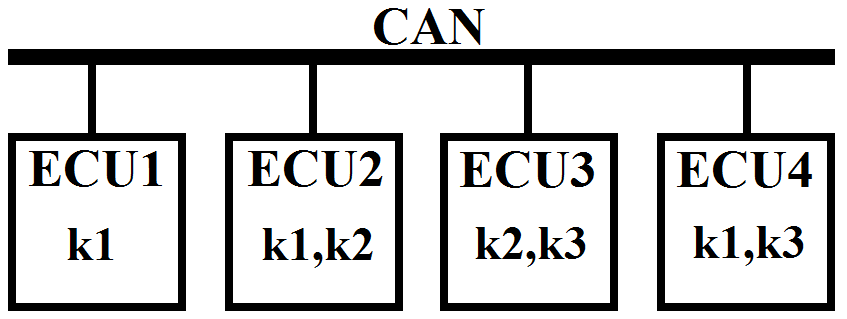
\includegraphics[width=\columnwidth]{figures/key_distribution.png}
		\caption{Mini-MAC key distribution.  Each group of ECUs shares an authentication key.}
		\label{fig-key}
	\end{figure}
	
\subsection{Design}
\label{design}

	\begin{figure}
		\centering
		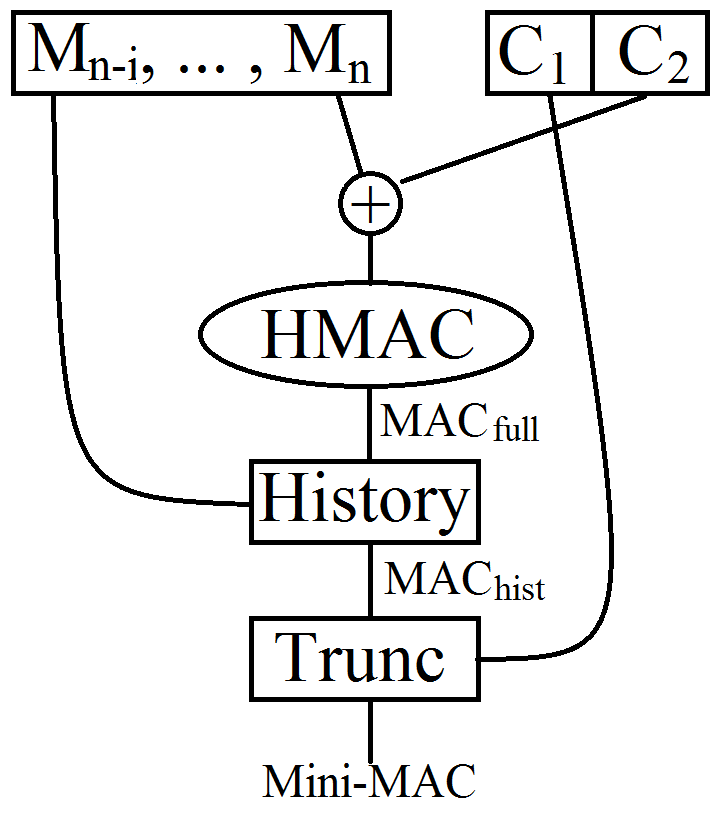
\includegraphics[width=\columnwidth]{figures/minimac_diagram.png}
		\caption{Mini-MAC. The Mini-MAC of a message $M_n$ is a truncated HMAC of 
		the XOR of $M_n$, a counter, and the most recent $i$ messages.}
		\label{fig-minimac}
	\end{figure}

Figure~\ref{fig-minimac} shows how to compute 
$Mini\hbox{-}MAC(k,M_n,s,C,\hbox{History})$, 
where $k$ is the group key, 
$M_n$ is the current message, 
$s$ is the number of available bits in the current CAN frame, 
$C$ is the message counter, 
and $\hbox{History} = (M_{n-{\lambda}}, \ldots, M_{n-1})$ is the sequence of the most recent
$\lambda$ messages.

The Mini-MAC tag is computed as

\begin{equation}
\text{MAC}_{\text{mini}} = \hbox{trunc(}s,\text{HMAC}(k,\text{Input})),
\end{equation}

\noindent where HMAC is the underlying HMAC and $\hbox{trunc}(s,\cdot)$
extracts $s$ bits from its input.  The input to HMAC is computed as

\begin{equation}
\text{Input} = M_n \oplus C \oplus (M_{n-{\lambda}} \oplus \cdots \oplus M_{n-1}) .
\end{equation}


%\begin{equation}
%\text{For }i=1:h\text{, MAC}_\text{hist} = \text{MAC}_{\text{full}}\oplus\text{Message}_{n-i}
%\end{equation}
%
%\begin{equation}
%\text{MAC}_{\text{mini}} = \text{MAC}_{\text{full}}(l,l+s)
%\end{equation}


\subsection{Implementation}
\label{implementation}

We implemented Mini-MAC using three different component hash functions (MD5, SHA-1, and SHA-2) to compare the resulting running times.  
Each group key is 128~bits.  The $\hbox{trunc}(s,\cdot)$ function extracts the first $s$ bits of its input.

We recommend a 64-bit counter, which (assuming at most 40 message per second) ensures no repeated counter state for 20 years
of continuous operation (32 bits would prevent counter roll-over for 20 years with four hours of driving a day).

%Assuming continuous operation (that is every second for 20 years) at 40 messages / second, roughly 25 billion messages will be exchanged. A 35-bit counter %will cover roughly 35 billion messages, but to cover that extreme use pattern, a 64-bit counter would be the smallest "standard" size counter. However, a %32-bit counter would cover 4 hours of driving a day, every day, for 20 years. 

For \textbf{HMAC-MD5},
we adapted Peslyak's~\cite{Peslyak} implementation of MD5~\cite{MD5} for the MSP430 platform, producing a 128-bit output. 
Despite known collision attacks on MD5~\cite{Wang-MD5}, we consider
MD5 for Mini-MAC for its very fast speed.  [the relevant attack here is known pre-image, not
collision finding.  more in security section]

For \textbf{HMAC-SHA-1},
we adapted Conte's~\cite{Conte-SHA1} SHA-1~\cite{FIPS-180-4} implementation for the MSP430 platform, producing a 160-bit output. 
As for MD5, despite known security vulnerabilities in SHA-1 \cite{Wang-SHA1}, 
we consider SHA1 as a potential candidate.

For \textbf{HMAC-SHA-2},
we also adapted Conte's~\cite{Conte-SHA256} SHA-2-256 implementation for the MSP430 platform, producing a 256-bit output. 
A member of the SHA-2 family of hash functions, SHA-2 is still in use and is recommended by NIST as a cryptographic hash function, 
though SHA-3 will soon replace it\cite{FIPS-180-4}. We did not use SHA-3 because we did not find an implementation of it
for the MSP430.  Throughout, we shall refer to SHA-2-256 as SHA-2.